
\begin{figure*}[t]
    \centering
    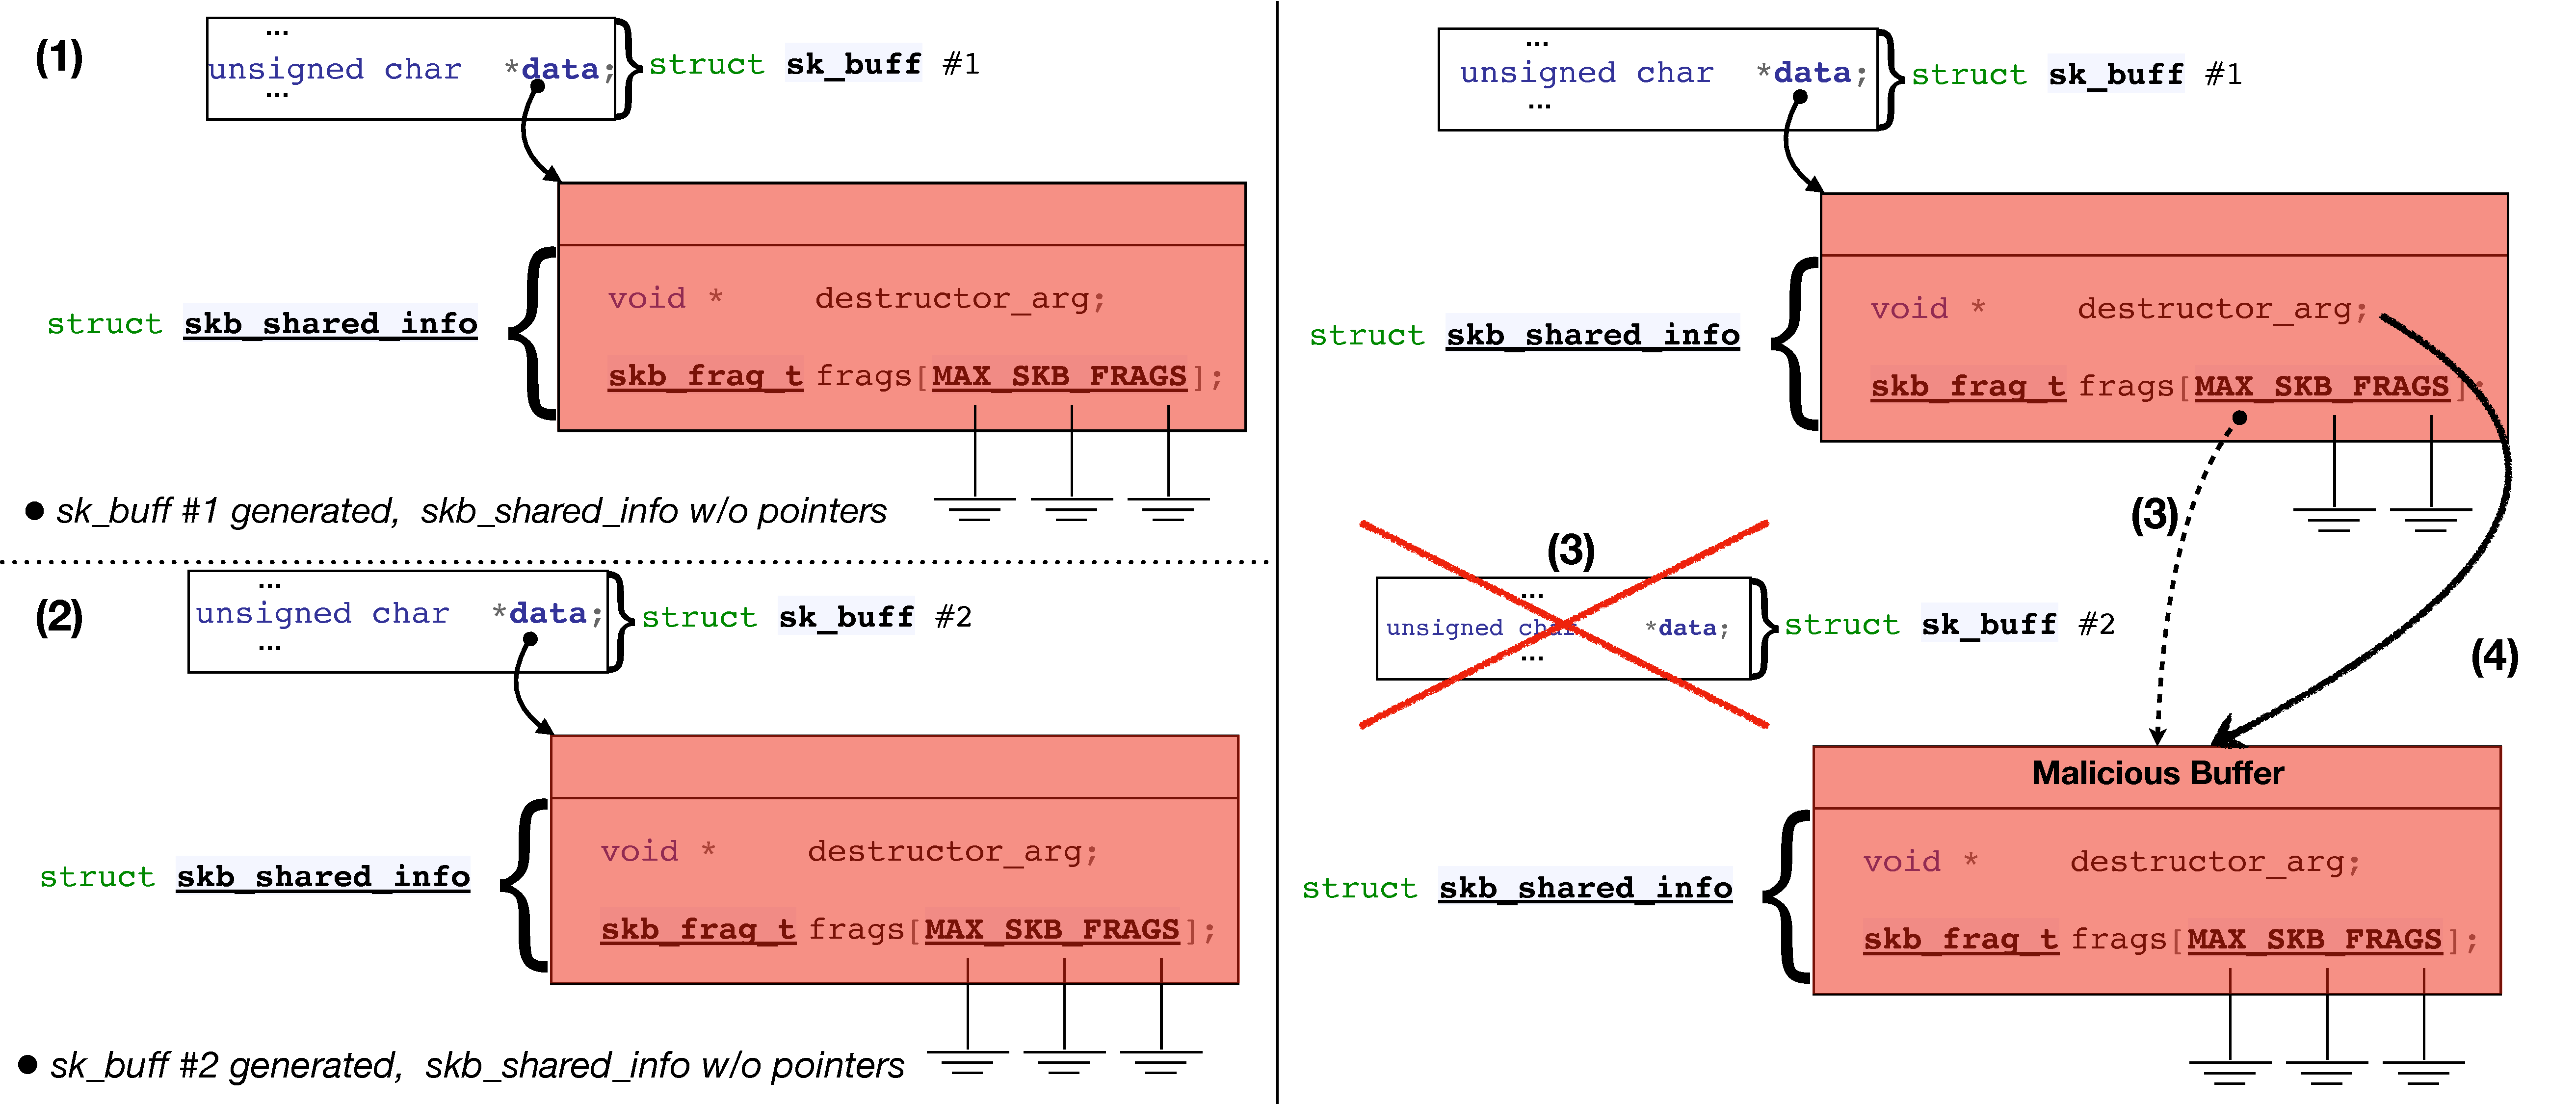
\includegraphics[width=\linewidth]{figs/gro.pdf}
    \caption{An RX \skb{} after GRO provides the \kva{} for a DMA attack.}
    \label{fig:gro_xdp}
\end{figure*}

%\section{Additional Compound attacks}\label{appx:additional_compound}

% \subsection{\textbf{eXpress Data Path}}\label{sec:xdp}

% eXpress Data Path (XDP)~\cite{xdp} provides a way for users to add custom handling to RX buffers with little overhead. Common use cases include DDOS mitigation, forwarding and load balancing. To support the latter, the RX buffers are mapped with BIDIRECTIONAL access to the NIC. 

% The tg3 driver does not support XDP. XDP support is usually added to high-speed NICs, such as ConnectX-4 (mlx5\_core). Accordingly, in this attack, we focus on the mlx5\_core driver, which, as mentioned in Sec, \ref{sec:forward}, does not unmap the RX buffers and reuses the pages using the page\_pool mechanism \cite{page_pool}. Subsequently, these pages are never unmapped, and remain accessible to the device for both reading and writing. 

% The fact that the NIC has both read and write access to \shinfo, allows the NIC to execute an attack in 4 steps (Fig. \ref{fig:gro_xdp}):
% \begin{enumerate}
%     \item An RX TCP packet is generated. Then, the \shinfo{} is initialised by the driver and the \texttt{frags} are filled with NULL pointers. Finally, the packet is handed to the next layer.

%     \item A second RX \skb{} is generated as part of the same TCP stream, initialized and also handed to the next layer.

%     \item Both packets reach the GRO layer. Then, the second \skb{} is coalesced with the first packet, the \skb{} is freed and the \data{} is added as a \texttt{frag} to the first \skb.

%     \item The NIC reads the updated \texttt{frag} field and translates the \page{} address to a valid \kva{}. Finally, the device fills the \texttt{destructor\_arg} field, creating a poisoned \skb{} (Fig. \ref{fig:sh_info}).
% \end{enumerate}

% The difference between this flow and a regular receive flow is the additional read capability the NIC has due to XDP. That is, the last step, where \kva is obtained, is possible only due to the additional READ access.

% \smallskip
% \noindent\textbf{Remark.} Other drivers that have XDP support, also tend to map RX buffers with BIDIRECTIONAL (e.g., bnxt, i40e, mlx4\_en). Interestingly, the mlx5\_core driver has two modes of operation: (1) linear - where an skb is built around an RX buffer and, (2) non-linear where the driver is filling up the \texttt{frags} of \shinfo, which was never mapped. The former is the default, and the later is actually secure. The non-linear mode is secure because \shinfo{} is \emph{never} accessible to the device. Thus the NIC never gains the oportunity to attack.

\subsection{Forward Thinking \Compound \DIFdelbegin \DIFdel{attack}\DIFdelend \DIFaddbegin \DIFadd{Attack}\DIFaddend }\label{appx:additional_compound}


Packet forwarding is a standard Linux feature that allows a Linux machine to serve as a router or a load balancer. Packet forwarding functionality is usually disabled by default on Linux servers.

When this functionality is enabled, the NIC can independently generate an RX packet to a legitimate destination. This packet will then be forwarded to become a TX packet. However, unlike \DIFdelbegin \DIFdel{in }\DIFdelend the TCP layer\DIFdelbegin \DIFdel{that }\DIFdelend \DIFaddbegin \DIFadd{, which }\DIFaddend usually creates \skb{} packets with fragments, device drivers often create a linear \skb{}. Namely, the drivers do not fill the \texttt{frags}, which the attacker uses to obtain a \kva. Device drivers, use the \DIFdelbegin %DIFDELCMD < \\%%%
\DIFdelend \texttt{napi\_gro\_receive} function to pass the \skb{} to the upper layer\DIFdelbegin \DIFdel{(this }\DIFdelend \DIFaddbegin \DIFadd{. This }\DIFaddend is the standard for most NIC drivers\footnote{\DIFdelbegin \DIFdel{Used }\DIFdelend \DIFaddbegin \DIFadd{It is used }\DIFaddend by 98 NIC drivers \DIFdelbegin \DIFdel{, }\DIFdelend in Linux 5.0}). 

In this case, the upper layer is the Generic Receive Offload (GRO) layer \cite{gro}. \DIFaddbegin \DIFadd{The }\DIFaddend GRO attempts to aggregate multiple TCP segments into a single large packet. Specifically, \DIFaddbegin \DIFadd{the }\DIFaddend GRO converts multiple linear \skb{} buffers \DIFdelbegin \DIFdel{(}\DIFdelend belonging to a single TCP stream\DIFdelbegin \DIFdel{) }\DIFdelend \DIFaddbegin \DIFadd{, }\DIFaddend into a single \skb{} with multiple fragments. This \skb{} then traverses the Linux network stack and becomes a TX packet. The attacker can use this TX packet as described in the previous attack \DIFdelbegin \DIFdel{(Fig. }\DIFdelend \DIFaddbegin \DIFadd{shown in Figure }\DIFaddend \ref{fig:payload}).

Packet forwarding, also opens up an additional attack option. An attacker \DIFdelbegin \DIFdel{might }\DIFdelend \DIFaddbegin \DIFadd{may }\DIFaddend be interested in persistent surveillance rather than overtaking the machine. \DIFdelbegin %DIFDELCMD < 

%DIFDELCMD < %%%
\DIFdelend Packet forwarding allows the NIC to inspect arbitrary pages at will. 
Instead of sending a TCP packet and letting the GRO layer fill in the \texttt{frags} information, the NIC can generate a small UDP packet and fill in the \texttt{frags} array with any arbitrary \page{} addresses within the system. \DIFdelbegin \DIFdel{This results in the mapping of these pagesby the driver}\DIFdelend \DIFaddbegin \DIFadd{As a result, the driver maps these pages}\DIFaddend , providing READ access to \DIFaddbegin \DIFadd{the NIC for }\DIFaddend any page in the system\DIFdelbegin \DIFdel{to the NIC}\DIFdelend . 


To avoid detection and preserve OS stability, the device must undo the changes to \shinfo{} before creating a TX completion. That is, before letting the CPU know that the packet was sent and its buffer can now be freed. Otherwise, the OS will try freeing the pages, indicated by \shinfo.


